\hypertarget{matrices_8c}{
\section{matrices.c File Reference}
\label{matrices_8c}\index{matrices.c@{matrices.c}}
}
{\tt \#include $<$stdio.h$>$}\par
{\tt \#include $<$string.h$>$}\par
{\tt \#include \char`\"{}matdata.h\char`\"{}}\par
{\tt \#include \char`\"{}matrixmap.h\char`\"{}}\par


Include dependency graph for matrices.c:\begin{figure}[H]
\begin{center}
\leavevmode
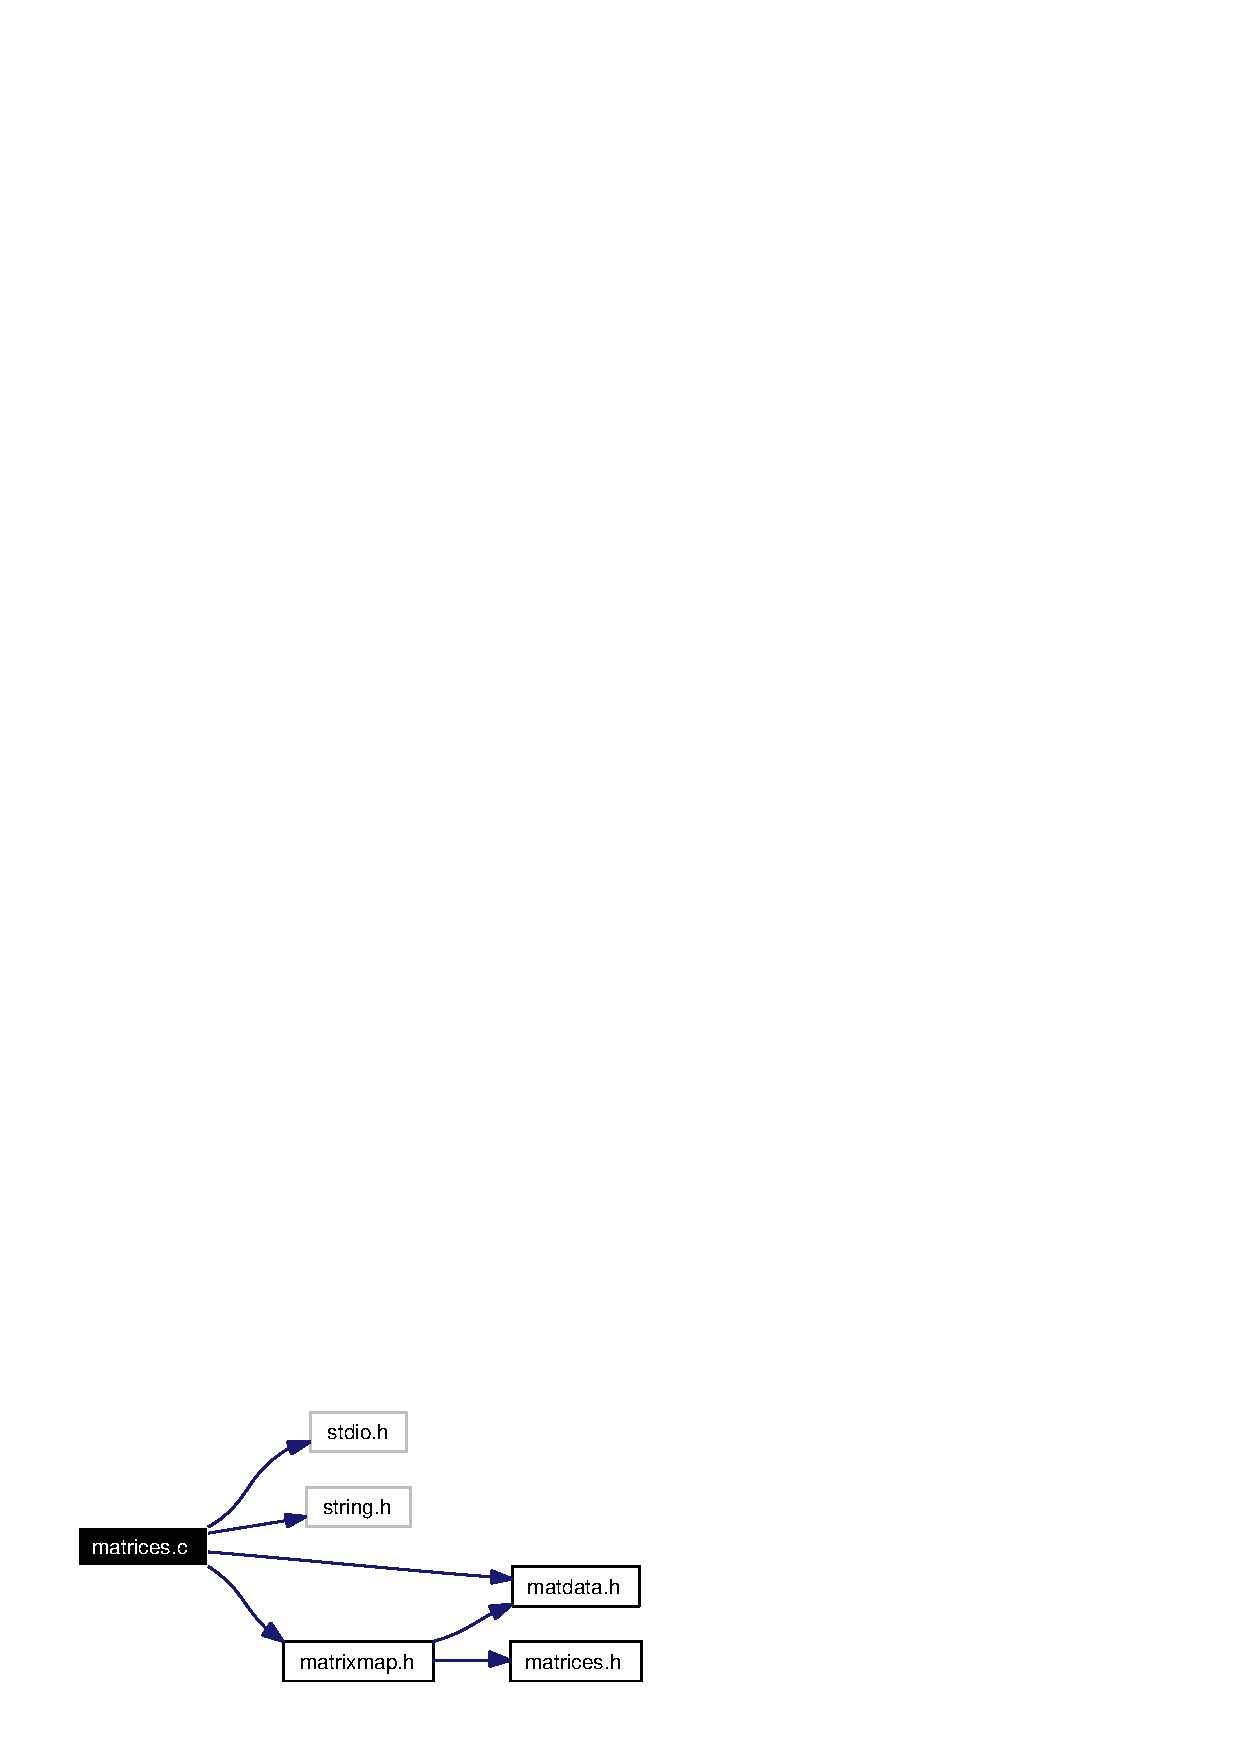
\includegraphics[width=154pt]{matrices_8c__incl}
\end{center}
\end{figure}
\subsection*{Defines}
\begin{CompactItemize}
\item 
\#define \hyperlink{matrices_8c_a0}{DEFAULT\_\-MATRIX}~\hyperlink{matrices_8h_a12}{blosum62}
\end{CompactItemize}
\subsection*{Functions}
\begin{CompactItemize}
\item 
void \hyperlink{matrices_8c_a1}{get\-Matrix\-By\-Name} (char \hyperlink{matrixmap_8h_a0}{name}\mbox{[}$\,$\mbox{]}, const int($\ast$$\ast$matp)\mbox{[}MATRIX\_\-SIZE\mbox{]})
\end{CompactItemize}


\subsection*{Detailed Description}
This file contains functions for handling scoring matrices used for the sequence based Gemoda.

Definition in file \hyperlink{matrices_8c-source}{matrices.c}.

\subsection*{Define Documentation}
\hypertarget{matrices_8c_a0}{
\index{matrices.c@{matrices.c}!DEFAULT_MATRIX@{DEFAULT\_\-MATRIX}}
\index{DEFAULT_MATRIX@{DEFAULT\_\-MATRIX}!matrices.c@{matrices.c}}
\subsubsection[DEFAULT\_\-MATRIX]{\setlength{\rightskip}{0pt plus 5cm}\#define DEFAULT\_\-MATRIX~\hyperlink{matrices_8h_a12}{blosum62}}}
\label{matrices_8c_a0}




Definition at line 7 of file matrices.c.

Referenced by get\-Matrix\-By\-Name().

\subsection*{Function Documentation}
\hypertarget{matrices_8c_a1}{
\index{matrices.c@{matrices.c}!getMatrixByName@{getMatrixByName}}
\index{getMatrixByName@{getMatrixByName}!matrices.c@{matrices.c}}
\subsubsection[getMatrixByName]{\setlength{\rightskip}{0pt plus 5cm}void get\-Matrix\-By\-Name (char {\em name}\mbox{[}$\,$\mbox{]}, const int $\ast$$\ast$ {\em matp}\mbox{[}MATRIX\_\-SIZE\mbox{]})}}
\label{matrices_8c_a1}


A simple function to take the matrix name argument given as input to gemoda and return the physical memory location of that matrix by using the matrix\_\-map construct. Input: a string containing the matrix name a pointer to a two-dimensional array. Output: None, though the value of the pointer given as input is changed to reflect the location of the matrix

Definition at line 34 of file matrices.c.

References DEFAULT\_\-MATRIX, and matrix\_\-map.

\scriptsize\begin{verbatim}35 {
36   int i;
37   for (i = 0; matrix_map[i].name != NULL; i++)
38     {
39       if (strcmp (name, matrix_map[i].name) == 0)
40     {
41       break;
42     }
43     }
44   if (matrix_map[i].name != NULL)
45     {
46       *matp = (matrix_map[i].mat);
47     }
48   else
49     {
50       *matp = (DEFAULT_MATRIX);
51     }
52 }
\end{verbatim}
\normalsize 


